\chapter{Dataset Exploration}
\label{chapter:dataset}

In order to leverage the dataset \cite{7k-books} used in the recommender system, it has to go through preprocessing steps necessary to enable meaningful analysis. 
All work was performed using Pythons \texttt{pandas}, \texttt{numpy}, and \texttt{matplotlib/seaborn} libraries, as defined in the data exploration script.

\section{Dataset Overview}
\label{sec:dataset-overview}

The initial dataset, \texttt{books.csv}, contains metadata for 6,810 books. It includes the following fields: \texttt{isbn13}, \texttt{isbn10}, \texttt{title}, \texttt{subtitle}, \texttt{authors}, \texttt{categories}, \texttt{thumbnail}, \texttt{description}, \texttt{published\_year}, \texttt{average\_rating}, \texttt{num\_pages}, and \texttt{ratings\_count}.

Some fields, such as \texttt{subtitle}, \texttt{thumbnail}, and \texttt{categories}, had significant missing values. The project focuses on the fields relevant for recommendation: \texttt{description}, \texttt{average\_rating}, \texttt{num\_pages}, \texttt{published\_year}, and \texttt{authors}.

\begin{itemize}
    \item \texttt{title} — Book title
    \item \texttt{authors} — Author(s)
    \item \texttt{description} — Natural language description (often from publisher blurbs)
    \item \texttt{average\_rating} — User rating score
    \item \texttt{num\_pages} — Page count
    \item \texttt{published\_year} — Year of publication
\end{itemize}

These attributes were chosen due to their utility in both preprocessing (e.g. filtering) and vector-based analysis.

---

\section{Cleaning and Filtering}
\label{sec:data-cleaning}

To ensure high-quality input for the NLP model, books with missing or unusable descriptions, ratings, publication years, or page numbers were removed. 
This resulted in a cleaned dataset, \texttt{books\_cleaned.csv}, containing 6,507 entries.

Two new features were engineered:

\begin{itemize}
    \item \textbf{missing\_description:} Binary indicator showing whether the description was missing.
    \item \textbf{age\_of\_book:} Computed as $2025 - \texttt{published\_year}$.
\end{itemize}

---

\section{Exploratory Analysis}
\label{sec:data-exploration}

Visual and statistical analysis was performed on the cleaned dataset:

\begin{itemize}
    \item A \textbf{correlation heatmap} (using Spearman correlation) highlights relationships between numerical features such as number of pages, age, and average rating.
    \item A \textbf{distribution plot of average ratings} showed a bell-shaped curve centered around 3.8–4.2. This distribution informed the design of filtering sliders in the UI.
    \item A \textbf{publication year histogram} highlighted a strong skew toward books published after 2000.
    \item A \textbf{top authors chart} visualized the most prolific authors in the dataset.
\end{itemize}

\subsection{Correlation Heatmap}
\begin{figure}[H]
    \centering
    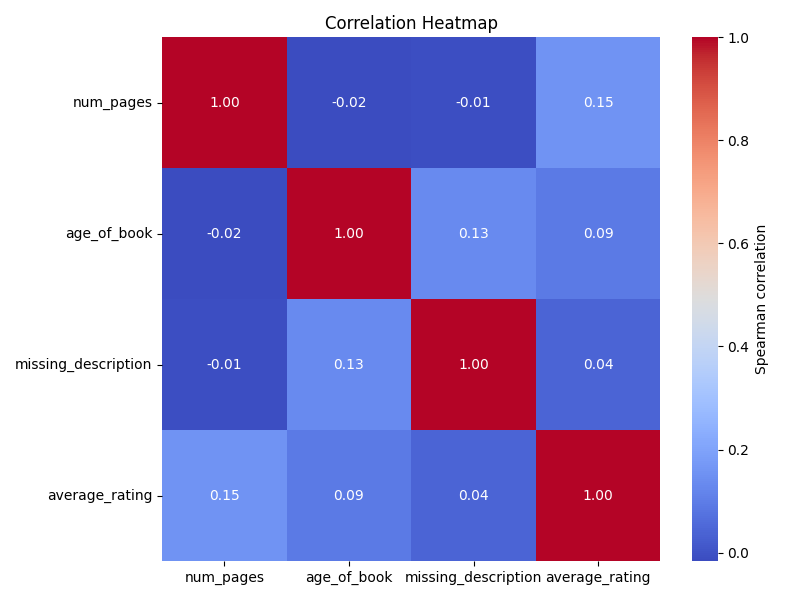
\includegraphics[width=0.7\textwidth]{figures/correlation_heatmap.png}
    \caption{Spearman Correlation Heatmap}
    \label{fig:correlation-heatmap}
\end{figure}

\subsection{Rating Distribution}
\begin{figure}[H]
    \centering
    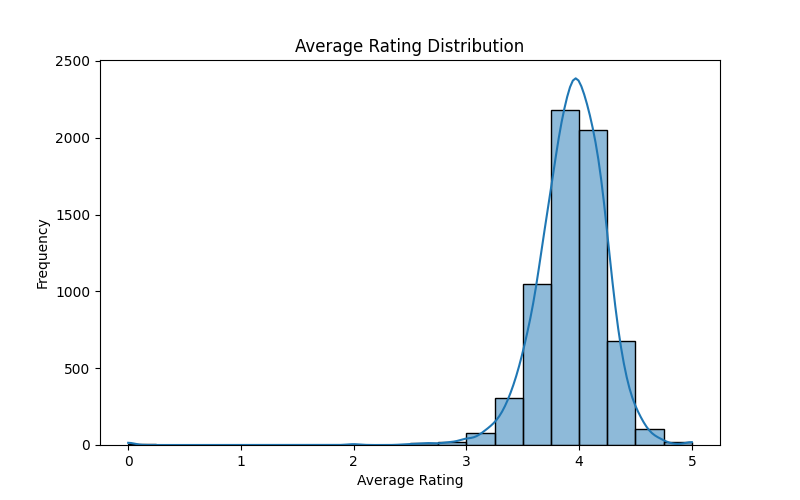
\includegraphics[width=0.7\textwidth]{figures/average_rating_distribution.png}
    \caption{Average Rating Distribution}
    \label{fig:rating-distribution}
\end{figure}

\subsection{Publication Year Distribution}
\begin{figure}[H]
    \centering
    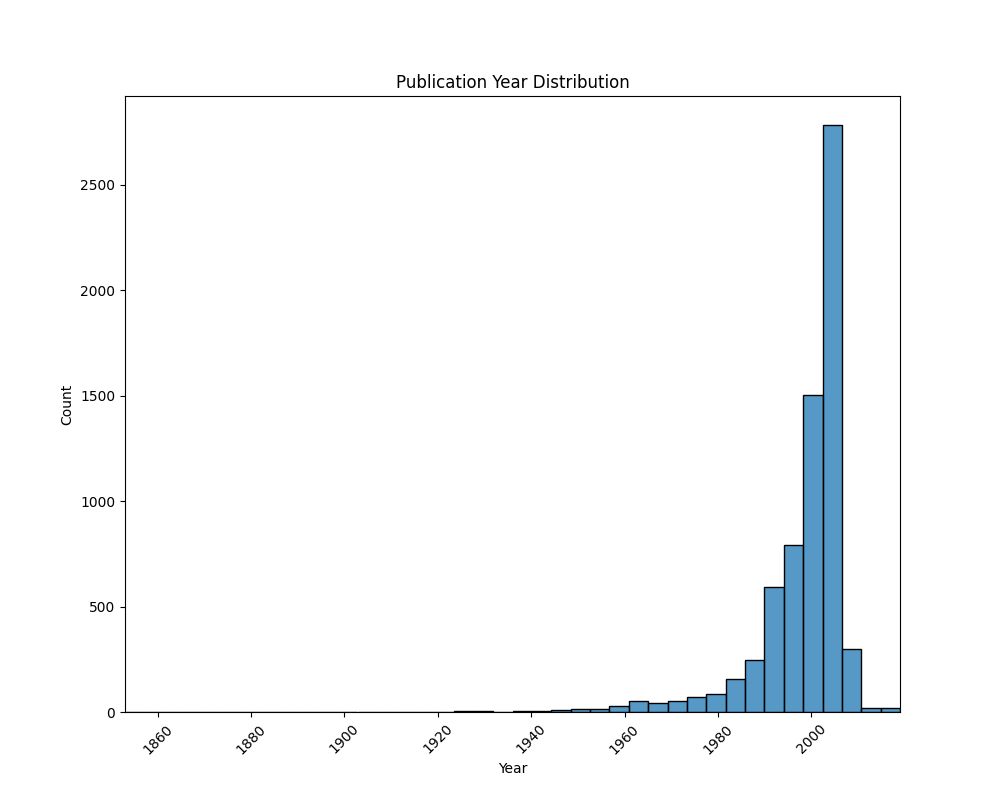
\includegraphics[width=0.7\textwidth]{figures/publication_year_distribution.png}
    \caption{Publication Year Distribution}
    \label{fig:pubyear-distribution}
\end{figure}

\subsection{Top Authors}
\label{sec:top-authors}
\begin{figure}[H]
    \centering
    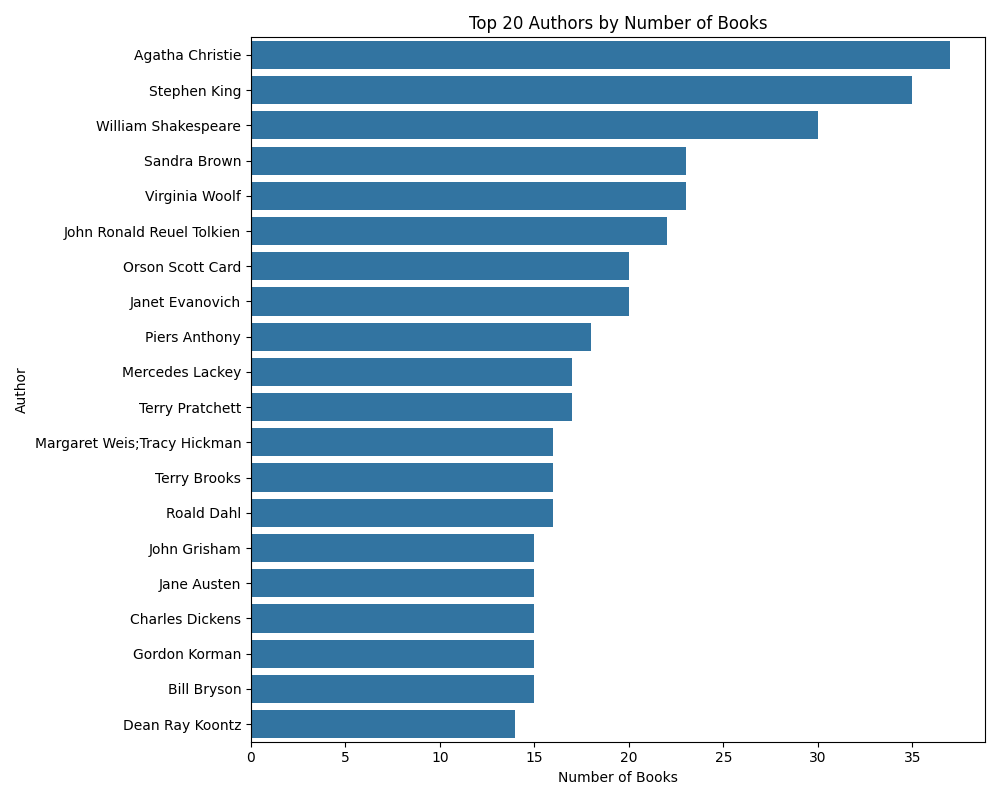
\includegraphics[width=0.8\textwidth]{figures/top_authors.png}
    \caption{Top 20 Authors by Number of Books}
    \label{fig:top-authors}
\end{figure}

These findings confirmed that the dataset was both large and diverse enough to support practical testing of the recommender system. 
Note that the heatmap in \autoref{fig:correlation-heatmap} shows weak correlation between all members, but the relative strongest between number of pages 
and the average rating. 
This may indicate that readers perceive longer books — particularly in fiction — as more substantial, potentially resulting in higher ratings.
Also that lower rated books are more rarely published and circulated widely, as seen in the histogram in \autoref{fig:rating-distribution}.